\centering
\begin{subfigure}[b]{0.45\textwidth}
    \centering
    % TikZ code for the first graph
    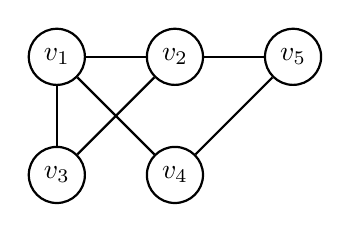
\begin{tikzpicture}[node distance={15mm}, thick, main/.style = {draw, circle}]
        \node[main] (1) {$v_1$};
        \node[main] (2) [right of=1] {$v_2$};
        \node[main] (3) [below of=1] {$v_3$};
        \node[main] (4) [below of=2] {$v_4$};
        \node[main] (5) [right of=2] {$v_5$};
        \draw (1) -- (2);
        \draw (1) -- (3);
        \draw (1) -- (4);
        \draw (2) -- (3);
        \draw (2) -- (5);
        \draw (4) -- (5);
    \end{tikzpicture}
    \caption{Undirected graph}
    \label{f_graphs_undirected}
\end{subfigure}
\begin{subfigure}[b]{0.45\textwidth}
    \centering
    % TikZ code for the second graph
    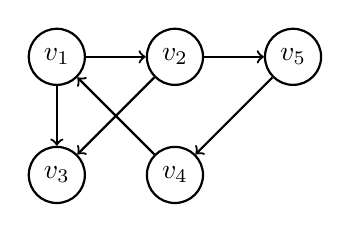
\begin{tikzpicture}[node distance={15mm}, thick, main/.style = {draw, circle}]
        \node[main] (1) {$v_1$};
        \node[main] (2) [right of=1] {$v_2$};
        \node[main] (3) [below of=1] {$v_3$};
        \node[main] (4) [below of=2] {$v_4$};
        \node[main] (5) [right of=2] {$v_5$};
        \draw[->] (1) -- (2);
        \draw[->] (1) -- (3);
        \draw[->] (4) -- (1);
        \draw[->] (2) -- (3);
        \draw[->] (2) -- (5);
        \draw[->] (5) -- (4);
    \end{tikzpicture}
    \caption{Directed graph}
    \label{f_graphs_directed}
\end{subfigure}
\par\bigskip
\begin{subfigure}[b]{0.45\textwidth}
    \centering
    % TikZ code for the first graph
    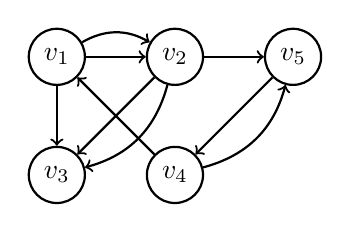
\begin{tikzpicture}[node distance={15mm}, thick, main/.style = {draw, circle}]
        \node[main] (1) {$v_1$};
        \node[main] (2) [right of=1] {$v_2$};
        \node[main] (3) [below of=1] {$v_3$};
        \node[main] (4) [below of=2] {$v_4$};
        \node[main] (5) [right of=2] {$v_5$};
        \draw[->] (1) -- (2);
        \draw[->] (1) to[bend left] (2);
        \draw[->] (1) -- (3);
        \draw[->] (4) -- (1);
        \draw[->] (2) -- (3);
        \draw[->] (2) to[bend left] (3);
        \draw[->] (2) -- (5);
        \draw[->] (5) -- (4);
        \draw[->] (4) to[bend right] (5);
    \end{tikzpicture}
    \caption{Multigraph}
    \label{f_graphs_multi}
\end{subfigure}
\begin{subfigure}[b]{0.45\textwidth}
    \centering
    % TikZ code for the second graph
    \begin{tikzpicture}[node distance={15mm}, thick, main/.style = {draw, circle}]
        \node[main] (1) {$v_1$};
        \node[main] (2) [right of=1] {$v_2$};
        \node[main] (3) [below of=1] {$v_3$};
        \node[main] (4) [below of=2] {$v_4$};
        
        \node[draw, rectangle, left=1mm of 1] {$f_{v_1}=[...]$};
        \node[draw, rectangle, right=1mm of 2] {$f_{v_2}=[...]$};
        \node[draw, rectangle, left=1mm of 3] {$f_{v_3}=[...]$};
        \node[draw, rectangle, right=1mm of 4] {$f_{v_4}=[...]$};
        
        \draw (1) -- (2);
        \draw (1) -- (3);
        \draw (4) -- (1);
        \draw (2) -- (3);
    \end{tikzpicture}
    \caption{Attributed graph}
    \label{f_graphs_attributed}
\end{subfigure}
\par\bigskip
\begin{subfigure}[b]{0.45\textwidth}
    \centering
    % TikZ code for the first graph
    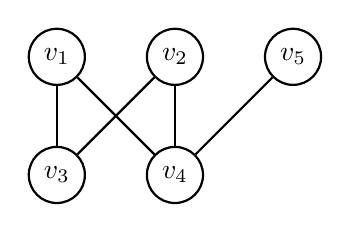
\begin{tikzpicture}[node distance={15mm}, thick, main/.style = {draw, circle}]
        \node[main] (1) {$v_1$};
        \node[main] (2) [right of=1] {$v_2$};
        \node[main] (3) [below of=1] {$v_3$};
        \node[main] (4) [below of=2] {$v_4$};
        \node[main] (5) [right of=2] {$v_5$};
        
        \draw (1) -- (3);
        \draw (1) -- (4);
        \draw (2) -- (3);
        \draw (2) -- (4);
        \draw (4) -- (5);
    \end{tikzpicture}
    \caption{Bipartite graph}
    \label{f_graphs_bipartite}
\end{subfigure}
\begin{subfigure}[b]{0.45\textwidth}
    \centering
    % TikZ code for the second graph
    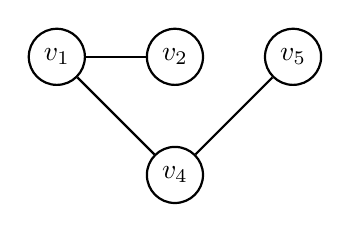
\begin{tikzpicture}[node distance={15mm}, thick, main/.style = {draw, circle}]
        \node[main] (1) {$v_1$};
        \node[main] (2) [right of=1] {$v_2$};
        \node[main] (4) [below of=2] {$v_4$};
        \node[main] (5) [right of=2] {$v_5$};
        \draw (1) -- (2);
        \draw (4) -- (1);
        \draw (5) -- (4);
    \end{tikzpicture}
    \caption{Subgraph of graph (a)}
    \label{f_graphs_subgraph}
\end{subfigure}